\documentclass{article}
\usepackage{graphicx}
\usepackage[margin=1.5cm]{geometry}
\usepackage{amsmath}

\begin{document}
\twocolumn

\title{Monday Reading Assessment: Unit 5, Power Consumption}
\author{Prof. Jordan C. Hanson}

\maketitle

\section{Memory Bank}

\begin{enumerate}
\item $\Delta E = P\Delta t$ ... Definition of power in terms of energy consumption, $\Delta E$, and time duration, $\Delta t$
\item 1 calorie = 4.184 Joules
\item 1 kcal = 4184 Joules
\item $\Delta U = m g \Delta y$ ... Change in gravitational potential energy
\end{enumerate}

\section{Power Consumption}

\begin{enumerate}
\item (a) What is the average useful power output of a person who does $6.00\times 10^6$ J of useful work in 8.00 hours? (b) Working at this rate, how long will it take this person to lift 2000 kg of bricks 1.50 m to a platform? (Work done to lift his body can be omitted because it is not considered useful output here.) \\ \vspace{4cm}
\item Consider Fig. \ref{fig:1} (top). (a) What fraction of total power consumption is required by the human brain? (b) How many Joules of energy does the brain require in a day (estimate)? (c) Convert this to calories, then kcal. \\ \vspace{3cm}
\item Consider Fig. \ref{fig:1} (bottom). (a) If you are caught in the cold, and begin to shiver, how many Joules of energy would you lose in 30 minutes? (b) Compare this to the amount of energy required to sit at rest (awake) for 30 minutes?  (c) What is the ratio of energies consumed by these two activities? \\ \vspace{3cm}
\item A large household air conditioner may consume 15.0 kW of power. What is the cost of operating this air conditioner 3.00 hours per day for 30.0 days if the cost of electricity is \$0.110 per kiloWatt hour?
\end{enumerate}
\begin{figure}
\centering
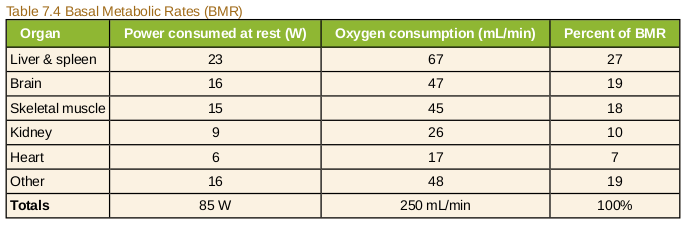
\includegraphics[width=0.49\textwidth]{figures/body2.png} \\
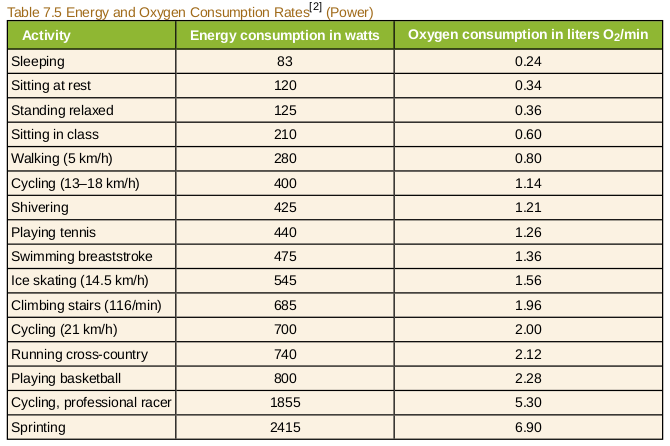
\includegraphics[width=0.49\textwidth]{figures/body3.png}
\caption{\label{fig:1} (Top) Metabolic rates of various physiological systems. (Bottom) Power consumption of various human activities.}
\end{figure}
\end{document}